%%%%%%%%%%%%%%%%%%%%%%%%%%%%%%%%%%%%%%%%%%%%%%%%%%%%%%%%%%%%%%%%%%
%%%%%%%% ICML 2013 EXAMPLE LATEX SUBMISSION FILE %%%%%%%%%%%%%%%%%
%%%%%%%%%%%%%%%%%%%%%%%%%%%%%%%%%%%%%%%%%%%%%%%%%%%%%%%%%%%%%%%%%%

% Use the following line _only_ if you're still using LaTeX 2.09.
%\documentstyle[icml2013,epsf,natbib]{article}
% If you rely on Latex2e packages, like most moden people use this:
\documentclass{article}

% For figures
\usepackage{graphicx} % more modern
%\usepackage{epsfig} % less modern
% \usepackage{subfigure}
\usepackage{subcaption}
\usepackage{multicol}

% For citations
\usepackage{natbib}

% For algorithms
\usepackage{algorithm}
\usepackage{algorithmic}

% For math
\usepackage{amsmath}
\usepackage{siunitx}

% As of 2011, we use the hyperref package to produce hyperlinks in the
% resulting PDF.  If this breaks your system, please commend out the
% following usepackage line and replace \usepackage{icml2013} with
% \usepackage[nohyperref]{icml2013} above.
\usepackage{hyperref}

% Packages hyperref and algorithmic misbehave sometimes.  We can fix
% this with the following command.
\newcommand{\theHalgorithm}{\arabic{algorithm}}

% Employ the following version of the ``usepackage'' statement for
% submitting the draft version of the paper for review.  This will set
% the note in the first column to ``Under review.  Do not distribute.''
\usepackage{icml2013}
% Employ this version of the ``usepackage'' statement after the paper has
% been accepted, when creating the final version.  This will set the
% note in the first column to ``Proceedings of the...''
% \usepackage[accepted]{icml2013}


% The \icmltitle you define below is probably too long as a header.
% Therefore, a short form for the running title is supplied here:
\icmltitlerunning{6.867: Final Project}

\begin{document}

\twocolumn[
  \icmltitle{6.867: Final Project}

  % % It is OKAY to include author information, even for blind
  % % submissions: the style file will automatically remove it for you
  % % unless you've provided the [accepted] option to the icml2013
  % % package.
  % \icmlauthor{Andrea Li}{liandrea@mit.edu}
  % \icmladdress{Your Fantastic Institute,
  %             314159 Pi St., Palo Alto, CA 94306 USA}
  % \icmlauthor{Tyson Chen}{ytchen33@mit.edu}
  % \icmladdress{Their Fantastic Institute,
  %             27182 Exp St., Toronto, ON M6H 2T1 CANADA}

  % You may provide any keywords that you
  % find helpful for describing your paper; these are used to populate
  % the "keywords" metadata in the PDF but will not be shown in the document

  \vskip 0.3in
]


\section{Introduction}
The NBA is currently one of the most popular sports in the world. Just a few months ago, over 30.8 million viewers tuned into watch Game 7 of the NBA finals between the Cleveland Cavaliers and the Golden State Warriors making it the third most viewed event in the U.S in 2016 (just behind the Super Bowl and the Academy Awards). As a result of this popularity, the betting market for the sport is enormous. NBA commissioner Adam Silver predicted the market to be around 400 billion dollars.

This report is concerned with exploring a variety of supervised learning techniques in hopes of being able to make predictions of game outcomes that are more accurate than the predictions made by NBA experts who set the betting line for each game. Before diving too deep into the algorithms, models, and predictions, we want to provide a quick overview of the structure of an NBA season as well as the various types of bets you can make in the NBA.

First, it is important to understand that the NBA is comprised of 30 teams split into two conferences (East and West). These 30 teams will each play 82 games across the regular season meaning that 1230 NBA games are played in total each season. For each game of the season, there are multiple bets that can be made. Below, we will discuss the two most common bets:

\textit{a) Win/ Loss:} This is the most basic bet that can be made. The gambler simply picks which team he believes will win the game and if he is correct then he'll win money.

\textit{b) The Spread:} The spread is a bit more advanced than simply win/loss. When a gambler bets against the spread, he either bets that the favorite shall win by more than the spread or that the underdog will lose by less than the spread. Typically, the spread is expressed as a negative number, which signifies the expected margin of victory for the favorite. In order to place a bet against the spread, a gambler generally needs to bet \$110 for the chance to win a \$100 payoff. The amount required for the chance to win \$100 is generally expressed in parentheses.
e.g. Golden State Warriors -7.4 (-110) \\
     Cleveland Cavaliers 7.4 (-110)

The gambling authority generally selects the spread with the goal of splitting the betting money down the line in order to essentially make arbitrage with 0 risk. Due to the fact that the spreads are created in this manner and not with accuracy in mind, we believe that there is definitely room for improvement

\section{Data collection}
For this project, we needed to gather a great deal of historical NBA game statistics in order to train our models. To collect season data, we primarily used publicly available data from \texttt{http://basketballvalue.com/downloads.php}.
These datasets contained time series data in the form of matchup logs for all NBA games ranging from 2005 to 2012. Matchup logs basically describe the interactions that occur between 5-person units. A new entry is created every time a substitution is made in a game. Through running a python script on these matchup logs, we were able to derive and construct a variety of statistics that would later serve as features. For seasons 2005-2008, the matchup logs were a bit simpler, so we were only able to derive basic statistics including points allowed and points scored (see \textit{table 1}). The matchup logs became a bit more advanced in seasons 2008-2011, which allowed us to derive more sophisticated statistics including offensive and defensive (see \textit{table 2}). Note that while we had data for the 2011-2012 season we ultimately decided not to use the data because a lockout occurred during this season which shortened the season to 66 games.

\begin{table}
  \begin{center}
    \begin{tabular}{ | c | c |}
      \hline
		Avg. points scored/ game & Avg. points allowed/game  \\ \hline
		Games played & Win rate        \\ \hline
		Avg. home court points scored   & Avg. home court points allowed        \\ \hline
		Home court games played   & Home court win rate      \\ \hline
		ELO & Home court advantage\\ \hline
    \end{tabular}
  \end{center}
  \caption{Basic statistics}
\end{table}

\begin{table}
  \begin{center}
    \begin{tabular}{ | c | c |}
      \hline
		Avg. defensive rebounds/ game & Avg. offensive rebounds/ game  \\ \hline
		Avg. possessions/ game & N/A       \\ \hline
    \end{tabular}
  \end{center}
  \caption{Advanced statistics}
\end{table}


For all seasons, we also constructed a new feature called ELO that is basically a reflection of a team's performance taking into account strength of schedule. What this means is that if two teams possess identical records, one of the teams may actually have a higher ELO score if they had to face stronger competition. In our literature review, this was not a feature that had been incorporated before in machine learning so we were particularly excited about its implications.

Many of the features generated for training and testing our predictor were derived from this game data. In order to create a general proxy for how strong a team was, we calculated running averages of points allowed, points scored, win rate, ELO, etc. and used these as input features to our classifier. These running averages were initialized to equal numbers for all teams at the beginning of the season and were subsequently updated as more data became available. Because these numbers were arbitrarily initialized to equal at the beginning of the season, however, running averages near the beginning of the season serve as less reliable data points, as outliers can significantly affect the running average.

These statistics were therefore plotted over time throughout the season in order to approximate when the running averages for each of these statistics stabilized to reliable averages. Example plots are given in Figures 1 and 2, in which the running average win rate and points scored for a given team is plotted over course of the season.

\begin{figure}[width=\linewidth]
\centering
  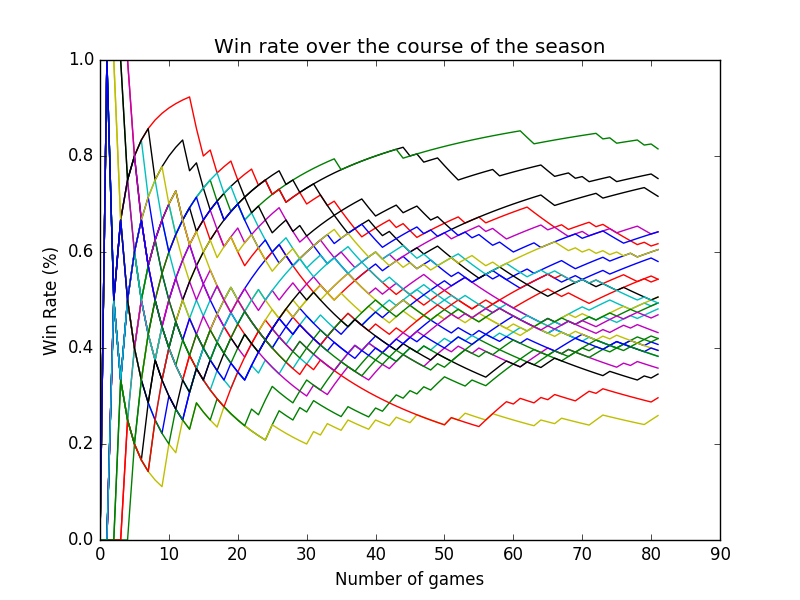
\includegraphics[width=1\linewidth]{code/figures/win_rate.png}
\caption{Win rate over time}
\end{figure}

\begin{figure}[width=\linewidth]
\centering
  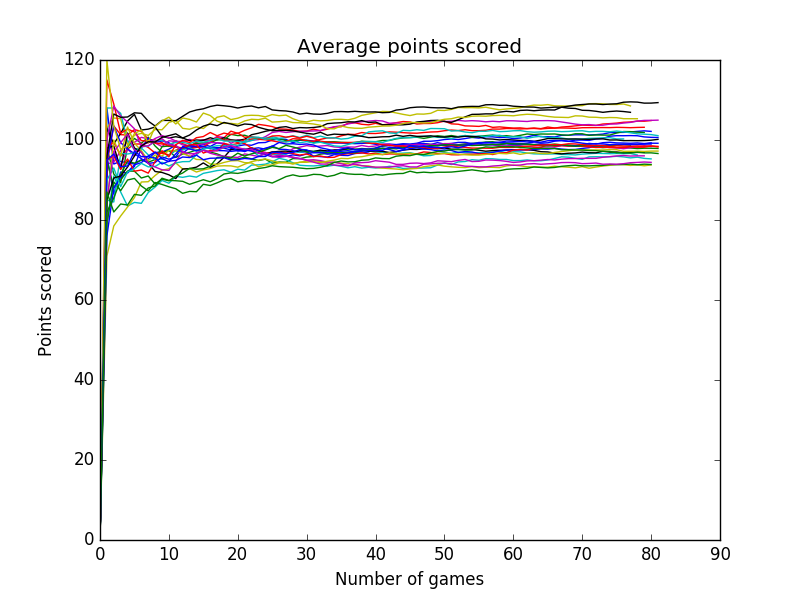
\includegraphics[width=1\linewidth]{code/figures/points_scored.png}
\caption{Points scored over time}
\end{figure}

In general, the running averages of the game data stabilized after approximately each team's twentieth game of the season (around the 1/4th mark of the season). When generating our training, validation, and test sets therefore, we only used data after each team's twentieth game in order to ensure that the features extracted from the data were representative of true team performance.

In order to compare our algorithm and our predicted spreads against Vegas and other betting authorities, we created a scraper to scrape relevant websites with both current and historical spreads. We primarily scraped this information from \texttt{http://www.sportsbookreview.com/betting-odds/} \texttt{nba-basketball/}.

\section{Normalization}
The need for feature normalization arises because our features are on different scales. For example, the average points a team scores every game is around $100$ whereas the average number of offensive rebounds a team gets per game is around $15$. In order to normalize the features we took a Z score approach that centered all the data at $0$ and set the standard deviation to be $1$.

\section{Linear classifier}
As a baseline, we used our own implementation of a linear classifier on basic features including running averages of home/away team points scored, points allowed, Elo score, games won, games played, and win rate. Based on the 2006-2007 season, in predicting win/loss (as opposed to the spread of a win/loss), the linear classifier had an accuracy of 64.3\% on training data and 63.3\% on testing data.

After adding further features, such as home court advantage, were added to the model, the linear classifier has an accuracy of 72.3\% on training data and 66.9\% on testing data based on the 2008-2009 season.

We additionally explored the ability of the classifier to predict spreads on games, in which the margin of victory is taken into account instead of a simple win/loss. In this case, the accuracy metric was the absolute value of the difference between the predicted spread and the actual spread. Using basic features on the 2006-2007 season, the average absolute value spread error was 9.31 points for training data and 10.07 points for testing data.

After adding further features, the average absolute value spread error decreased to 8.53 points for training data but increased to 13.60 points for testing data. This would imply that the classifier might be overfitting to the features that are provided as input to the algorithm, which would be expected for more complex architectures but was surprising in the context of the linear classifier explored here.

These results for the performance of the linear classifier are summarized in Table 1.
\begin{table}
  \begin{center}
    \begin{tabular}{ | c | c | c | }
      \hline
                      & Win/Lose Accuracy & Spread Error  \\ \hline
      Basic features  & 63.3\%            & 10.07         \\ \hline
      Extra features  & 66.9\%            & 13.60         \\ \hline
    \end{tabular}
  \end{center}
  \caption{Classifier performance on test dataset}
\end{table}

Similar results were found when we used a polynomial basis and allowed the degree of the polynomial fitting the data to grow. Out of values for $M \in [1, 10]$, we found that a regression model with $M=1$ performed best, where $M=10$ on the other side of the spectrum led to extreme overfitting. The average spread error is summarized in Table 2 for each of the different possible values for $M$, and graphs for representative values of $M$ are illustrated in Figure 3. Note that for ease of illustration of data here, only the win rate feature is used as the feature vector

\begin{table}
  \begin{center}
    \begin{tabular}{ | c | c | c | c | c | }
      \hline
      \textbf{M=1}    & \textbf{M=2}    & \textbf{M=3}     & \textbf{M=4}     & \textbf{M=5}      \\ \hline
      10.15  & 11.35  & 11.013  & 12.40   & 11.32    \\ \hline
      \textbf{M=6}    & \textbf{M=7}    & \textbf{M=8}     & \textbf{M=9}     & \textbf{M=10}     \\ \hline
      12.05  & 33.26  & 33.56   & 17.11   & 150.23   \\ \hline
    \end{tabular}
  \end{center}
  \caption{Average spread error for M values}
\end{table}

\begin{figure}[width=\linewidth]
\centering
\begin{multicols}{2}
  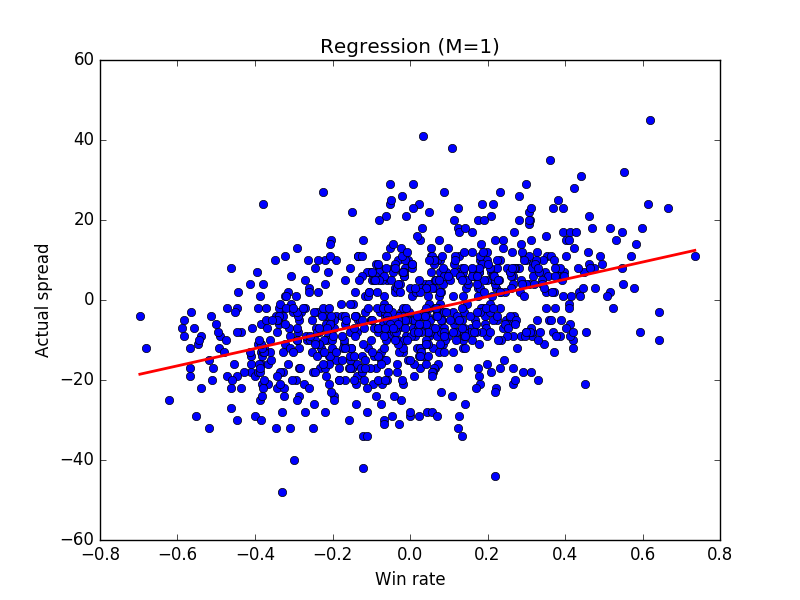
\includegraphics[width=1.2\linewidth]{code/figures/linear_regression(m=1).png}
  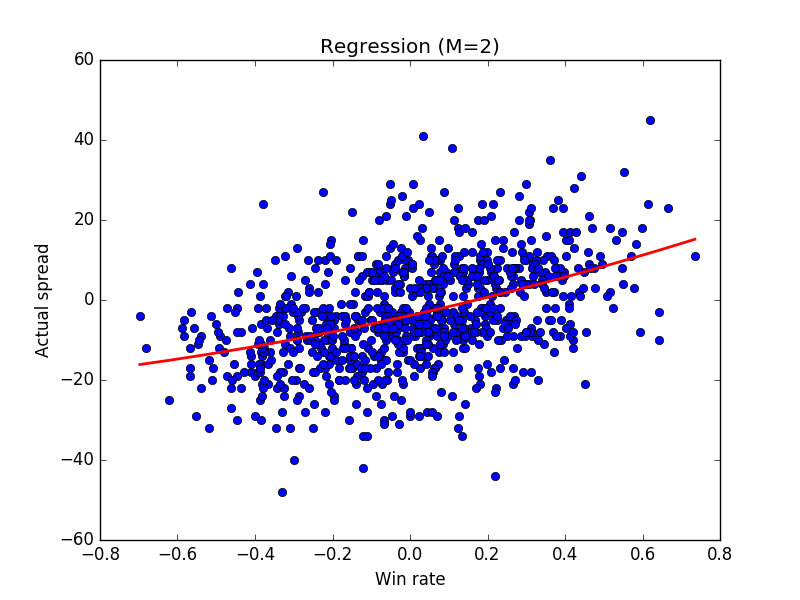
\includegraphics[width=1.2\linewidth]{code/figures/linear_regression(m=2).png}
  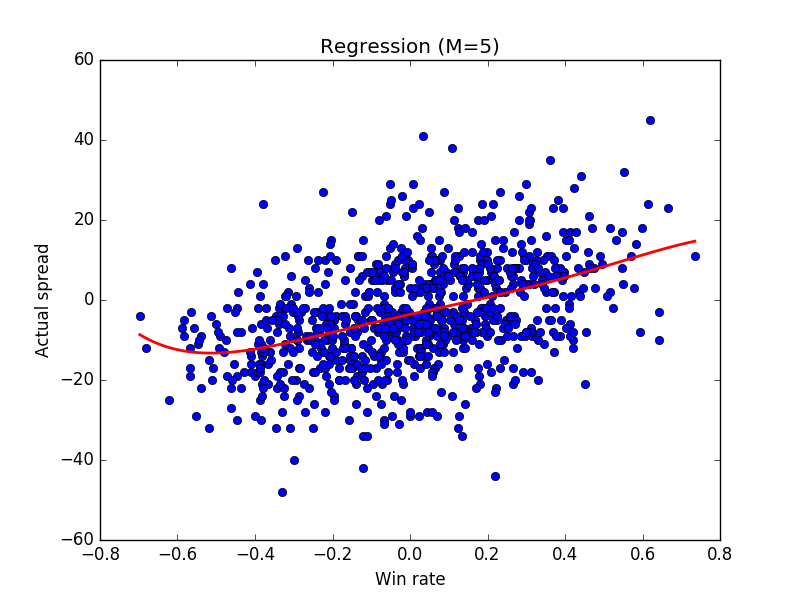
\includegraphics[width=1.2\linewidth]{code/figures/linear_regression(m=5).png}
  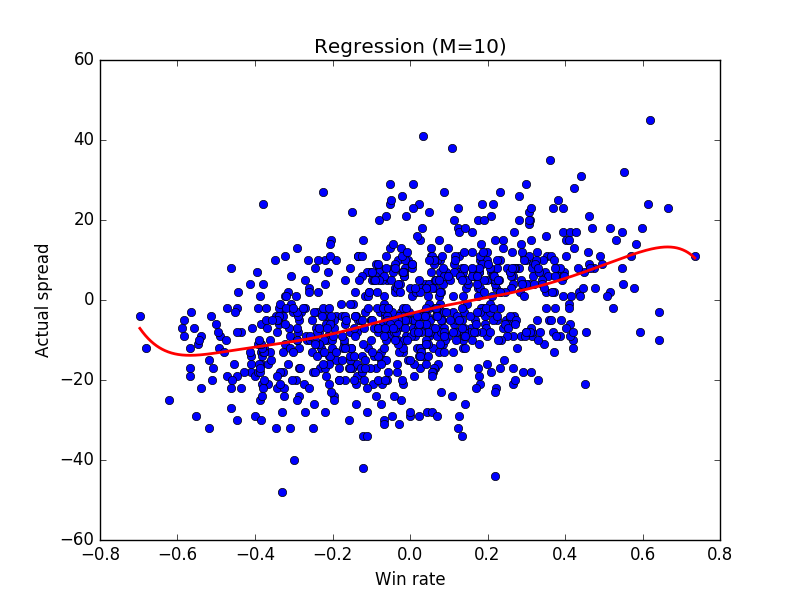
\includegraphics[width=1.2\linewidth]{code/figures/linear_regression(m=10).png}
\end{multicols}
\caption{Win rate vs. actual spread}
\end{figure}

We additionally explored the use of generating training, validation, and testing datasets across multiple seasons of data. In this case, because we train the model against certain features of the teams playing (e.g. running average win rate, average points scored, average points allowed, etc.), and not the skill level associated with the team itself, we can aggregate data across multiple seasons. This holds true even if teams and their respective players have changed significantly between seasons, because the features we draw from the data are running averages calculated from the season so far.

When we run the linear classifier on three seasons worth of data, in which the training, validation, and testing datasets are each made up of a season of data (about 1300 games), the accuracy of the algorithm improves as expected. More specifically, when run on three seasons of data, the linear classifier is able to classify win/loss of matchups with an accuracy of 72.3\% on training data and 68.6\% on testing data. In terms of spreads, the linear classifier predicts spreads with an average spread error of 8.98 points on training data and 9.29 points on testing data. Thus, increasing the size of the data set has a fairly significant improvement in the accuracy of the linear classifier when compared with the 66.9\% accuracy previously obtained for win/loss predictions and 13.60 spread error for spread predictions.

As previously mentioned, we explored classification of the linear classifier with a set of basic features and a set of more complex partially derived from these basic features. The basic features included each team's Elo score, average points scored, average points allowed, number of games played, number of games won, and win rate. The additional features we added included home court advantage (e.g. home court average points scored, home court average points allowed, home court win rate, etc.) as well as possessions, offensive rebounds, and defensive rebounds. In order to understand which features contributed most heavily to the win/loss and spreads predictions, we plotted the weights of each of the features. These relative weights are illustrated in Figure 4, in which the win rate features (away team win rate, home team win rate, away team home court win rate, and home team home court win rate) were in general the most important features. For three seasons of data however in win/loss predictions, the other features contributed much more relative to the classifiers for spreads predictions and one season of data.

\begin{figure}[width=\linewidth]
\centering
\begin{multicols}{2}
  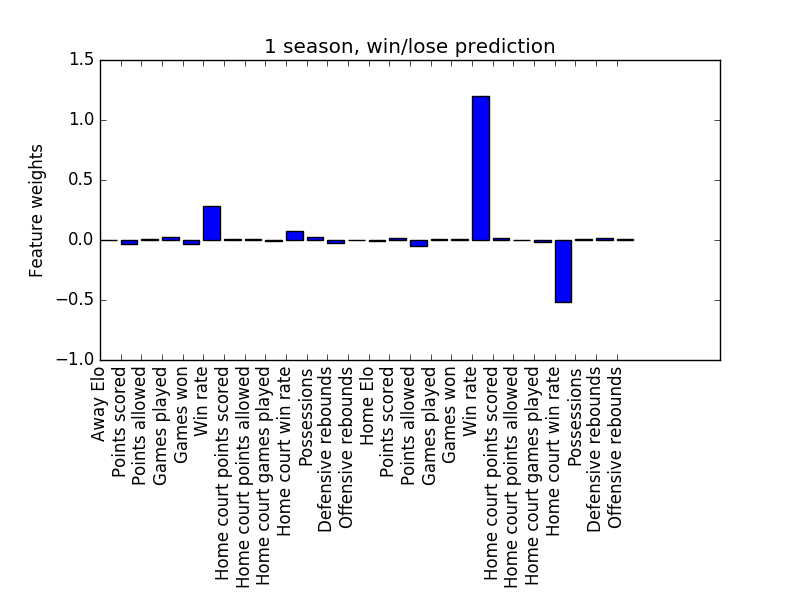
\includegraphics[width=1.2\linewidth]{code/figures/1season,winlose.png}
  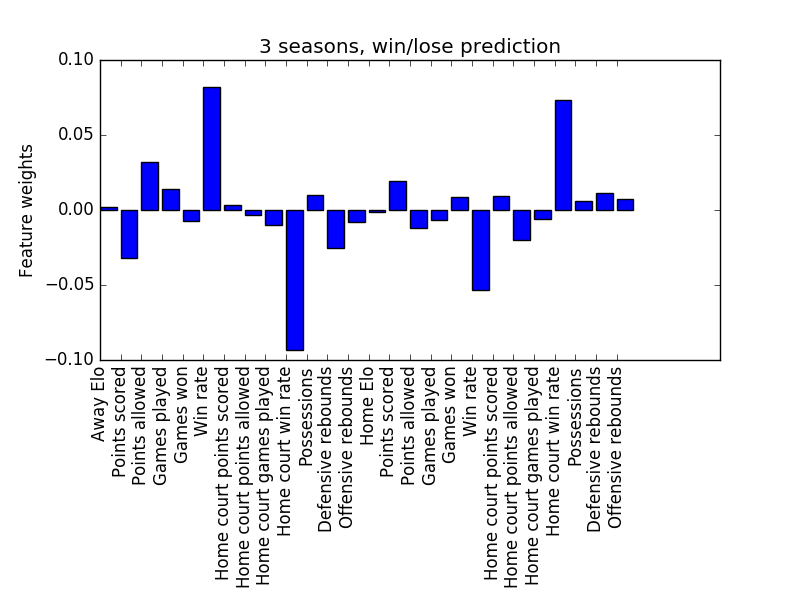
\includegraphics[width=1.2\linewidth]{code/figures/3seasons,winlose.png}
  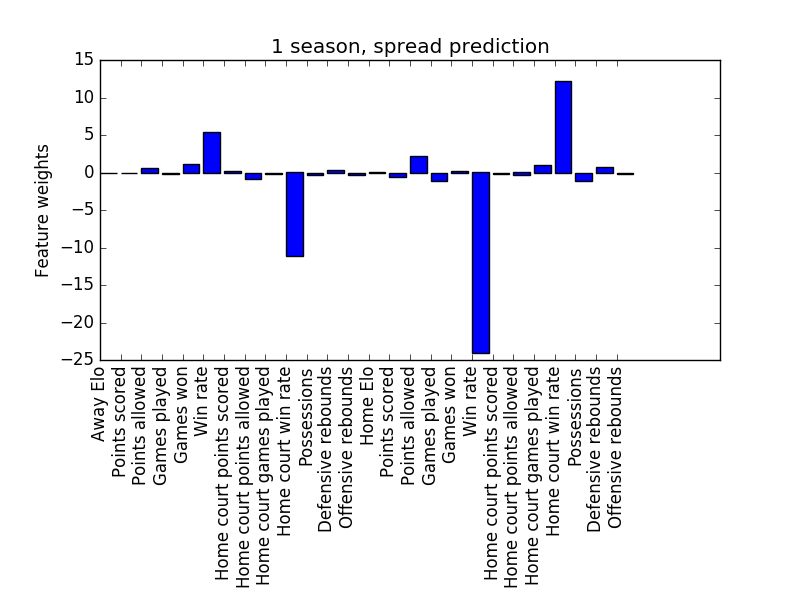
\includegraphics[width=1.2\linewidth]{code/figures/1season,spreads.png}
  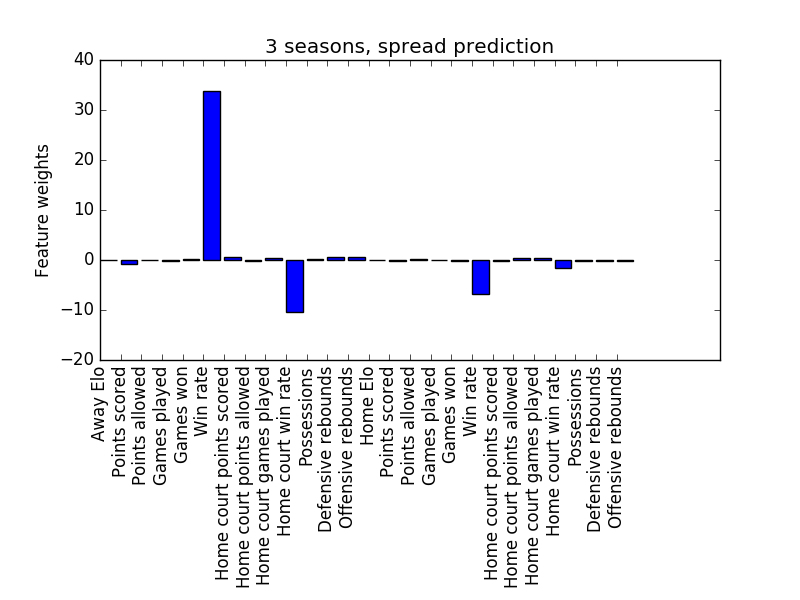
\includegraphics[width=1.2\linewidth]{code/figures/3seasons,spreads.png}
\end{multicols}
\caption{Linear classifier feature weights}
\end{figure}

Interestingly, when we train the linear classifier using only the win rate features, the classifier actually performs slightly better than with all the features. The numbers in Table 3 and 4 represent the accuracies and spread errors of the classifiers trained on all features and only win rate features when trained on one and three seasons of data, respectively. These findings seem to contradict the conclusions earlier in that adding more complex features such as home court advantage and rebounds improved the accuracy of the classifier. This could be due to overfitting to the number of features, especially in short periods of time in which averages might not necessarily be as representative of the overall skill level of a team.

\begin{table}
  \begin{center}
    \begin{tabular}{ | c | c | c | }
      \hline
                         & Win/Lose Accuracy & Spread Error  \\ \hline
      All features       & 66.9\%            & 13.6         \\ \hline
      Only win rate      & 70.7\%            & 8.95         \\ \hline
    \end{tabular}
  \end{center}
  \caption{Classifier performance on 1 season}
\end{table}

\begin{table}
  \begin{center}
    \begin{tabular}{ | c | c | c | }
      \hline
                         & Win/Lose Accuracy & Spread Error  \\ \hline
      All features       & 68.6\%            & 9.29         \\ \hline
      Only win rate      & 68.7\%            & 9.14         \\ \hline
    \end{tabular}
  \end{center}
  \caption{Classifier performance on 3 seasons}
\end{table}


\section{Evaluation}
In addition to calculating and analyzing the average spread error, we also compared our spreads predictions against other betting authorities' spreads. After creating a scraper which scraped the spreads posted by other betting authorities, we were able to determine the rate at which our spread would have beaten the betting authority's spread. This would occur in two scenarios: (1) if our predicted spread indicates that the winning team would have won by more than the other betting authority's predicted spread (e.g. if our spread is -8 and the other betting authority's spread is -5 on a game in which the favored team won by more than five points), or (2) if the predicted spread indicates that the winning team would have won by less or lost compared with theo ther begging authority's predicted spread (e.g. if our spread is +2 and the other betting authority's spread is -5 on a game in which the favored team lost or won by less than five points).


\section{Potential sources of failure}
Some drawbacks to the algorithm presented here include the fact that we do not examine individual player data. This was a choice made largely due to the fact that individualized player data is quite difficult to obtain, especially in quantities large enough for accurate training, validation, and testing. Because we look at a team's performance overall so far in the season however, this means that our algorithm is susceptible to changes in starting player lineups, player trades made during the season, and player injuries. Thus, despite the acceptable performance of our algorithm, we do identify this source of weakness in the ability to predict spreads and classify win/loss in matchups. Future iterations of the algorithm would therefore primarily seek to address these potential sources of failure in order to further improve and refine the overall predictive power of the algorithm.

\section{Neural Networks Approach}
After using a linear regression method to predict game outcomes as well as spreads, we next explored the use of neural networks for the very same problem. While we considered a multitude of neural networks at first, we ultimately decided to use a back-propagation multi-layer perceptron network provided by scikit learn for several reasons. First, the back-propagation aspect of the network allows us to perform supervised learning, which was our original goal. Secondly, the flexibility of this network made it very easy to change various hyperparameters such as the degree of regularization and the hidden layers size in order optimize for predictive capability. Finally, the network is able to perform both classification as well as regression, which enables us to make predictions for the two forms of bets that we are interested in.

\subsection{Design Decisions}
The relu activation function was the activation function of choice for the hidden layers because of sparsity as well as a reduced likelihood of vanishing gradients. For our weight optimization algorithm, we chose to use a batch gradient descent algorithm called the Limited-memory Broyden-Fletcher-Goldfarb-Shanno (LBFGS) algorithm in stead of a stochastic gradient descent (SGD) algorithm. The rational behind this design decision was due to the relatively small size of our dataset. With only 300/ 900 samples for each phase of classification we didn't really need the speed offered by SGD and empirically, we found LBFGS to be much more accurate. Because the weights of the network are initialized randomly we decided to also utilize a consensus based approach. For classification, this means that each prediction we make is actually the mode of the outcome of 7 predictions by the same neural network. Thus, if the neural network predicts the home team wins in 5 instances, and that the away team wins in 2 instances, we would predict that the home team wins. For regression, this means that each spread prediction we make is actually the mean of the outcome of 7 spreads made by the same neural network.

\subsection{Predicting win/loss}
As mentioned previously, predicting the winner of a particular NBA game boils down to a classification problem. 

\subsubsection{Training}
The input (X) to the multi-layer perceptron (MLP) classifier is a vector containing features for the two teams that are playing each other. At first, we utilized only the basic features but then we also incorporated the advanced features to see if we could improve performance. The Y values given to the classifier were either 1 (if the home team wins) or 0. Additionally, we tested our classifier on both 1 season of data (2008-2009) as well as 3 seasons of data (2008-2011). We also tested both normalized and un-normalized data and found that normalization had no impact on the ultimate accuracy of the classifiers. 

\subsubsection{Validation}
The purpose of validation is to determine the optimum hyperparameters for our neural network, which in our case is the regularization parameter as well as the size of the hidden layers. Through early testing/ experimentation it was discovered that hidden layers containing around 5-20 neurons performed the best so we incorporated that in creating our set of potential hidden layer sizes. Table 7 shows validation results for 3 seasons of data using both both basic and advanced features. The column headers are the hidden layer sizes (the $i^{th}$ number represents the number of hidden neurons in the $i^{th}$ hidden layer. The row headers are the various regularization coefficients we tried. Table 8 shows the aggregated validation results for classification.

\begin{table}
  \begin{center}
    \begin{tabular}{ | c | c | c | c | c | c | c |}
      \hline
            &             	(5,) & 	(10,) & 	(5,5) &  	(10,10) & 	(10,20,10) & 	(5,10,10,5)  \\ \hline
	0  &     	0.684 & 	0.671&	0.665&	0.683&	0.654&		0.671	    \\ \hline
	0.0001 &   0.589 &     \textbf{0.687}&	0.671&	0.673&	0.659&		0.669	    \\ \hline	
	0.01  &    	0.670 &     0.665&	0.589&	0.673&	0.653&		0.669	    \\ \hline	
	0.1	&	0.677&	0.672&	0.589&	0.676&	0.645&		0.680	    \\ \hline
	1&		0.675&	0.673&	0.665&	0.673&	0.669&		0.589	    \\ \hline
	
    \end{tabular}
  \end{center}
  \caption{Validation results for 2008-2011}
\end{table}

\begin{table}
  \begin{center}
    \begin{tabular}{ | c | c | c |}
      \hline
            &            	basic features & 	full features \\ \hline
	2008 season  &     	0.675 & 	0.704    \\ \hline
	2008-2011 seasons &   0.653&  0.687 \\ \hline	

	
    \end{tabular}
  \end{center}
  \caption{Aggregate validation results}
\end{table}

\subsubsection{Testing}
After finding the optimal architecture for our MLP classifier in each situation we proceeded to test the classifier on the testing data. The testing accuracies are depicted in table 9.

\begin{table}
  \begin{center}
    \begin{tabular}{ | c | c | c |}
      \hline
            &            	basic features & 	full features \\ \hline
	2008 season  &     	0.675 & 	0.693    \\ \hline
	2008-2011 seasons &   0.682&  0.679 \\ \hline	

	
    \end{tabular}
  \end{center}
  \caption{Aggregate validation results}
\end{table}


As you can see, through using a neural network approach we were able to derive slightly better results for classification compared to the linear regression approach. Additionally, we were able to get accuracies that were a bit higher than the previous ones found in literature (68 \%). 

\subsubsection{Overfitting}
When experimenting with various architectures for the neural network it was discovered that there was an interesting tradeoff between hidden layer complexity and testing accuracy, which highly resembled overfitting. 

\subsection{Predicting spreads}
As mentioned previously, predicting the spread of a particular NBA game boils down to a regression problem.

\subsubsection{Training}
The input (X) to the multi-layer perceptron (MLP) regressor is the exact same as the input to the classifier. The Y values, however, are now the actual realized spreads/ game outcomes (away team score - home team score). Just like for classification, we also tested our classifier on both 1 season of data as well as 3 seasons. Additionally, we also found that normalization had no impact on the performance of our predictor. 

\subsubsection{Validation}
When finding the optimal architecture for our MLP regressor we used two different approaches for validation, which optimized for different things. The first approach involved optimizing the neural network to predict spreads that minimized the average prediction error for each game. For example, if our regressor predicts that the home team would win be 4 points, but in fact the away team wins by 2 points that results in an error of 6 points for that game. The second approach was a more direct approach towards our ultimate goal of beating the spread. It involves optimizing the neural network to specifically beat the spread. For example, if the spread favors the home team by 4 points, and our predictor predicts the home team wins by 6 points , and the actual home team wins by 8 points then this is considered "beating the spread". Table 9 shows validation results (with approach 1) for 3 seasons of data using both both basic and advanced features.

\begin{table}
  \begin{center}
    \begin{tabular}{ | c | c | c | c | c | c | c |}
      \hline
            &             	(5,) & 	(10,) & 	(5,5) &  	(10,10) & 	(10,20,10) & 	(5,10,10,5)  \\ \hline
	0  &     	10.54 & 	9.52&	9.55&	9.50&	\textbf{9.44}&	10.54	    \\ \hline
	0.0001 &   9.56 &     	9.49&	9.56&	9.51&	9.51&		9.46	    \\ \hline	
	0.01  &    	9.55 &     	9.50& 	9.45&	9.51&	10.54&		9.46	    \\ \hline	
	0.1	&	9.47&	9.55 &	9.50&	9.53&	9.50&		9.45	    \\ \hline
	1&		9.52&	09.51&	10.54&	9.49&	9.58&		9.48	    \\ \hline
	
    \end{tabular}
  \end{center}
  \caption{Validation results for 2008-2011}
\end{table}

\subsubsection{Testing}


\section{Breakdown of individual work}
The breakdown of work between the two members of the group largely followed that given in the original project proposal. Andrea and Tyson jointly worked on preliminary review of the current techniques and the state of the art. Following this, Tyson was primarily involved in the collection of game data from past seasons, and Andrea created the scraper to collect data on historical spreads put out by various betting organizations on previous games. Andrea explored preliminary models such as linear regression, logistic regression, and regression with various basis functions and various degrees of regularization, and Tyson chiefly explored a neural network approach to predicting spreads and win/loss. As discussed during the project proposal meeting, we decided not to implement a convolutional neural network for this problem, as the architecture did not fit the structure of the problem as closely. We each tested the models we worked on against data test sets and historical spreads, and we split the writing up of the report equally.


\end{document}


% This document was modified from the file originally made available by
% Pat Langley and Andrea Danyluk for ICML-2K. This version was
% created by Lise Getoor and Tobias Scheffer, it was slightly modified
% from the 2010 version by Thorsten Joachims & Johannes Fuernkranz,
% slightly modified from the 2009 version by Kiri Wagstaff and
% Sam Roweis's 2008 version, which is slightly modified from
% Prasad Tadepalli's 2007 version which is a lightly
% changed version of the previous year's version by Andrew Moore,
% which was in turn edited from those of Kristian Kersting and
% Codrina Lauth. Alex Smola contributed to the algorithmic style files.
